\chapter{Cheating}

\section{Everyone is a cheater}
If A and B both are cheater one of them can report out of range values and none of them will get caught. In general, if all the node in the tree cheat then you can not detect.
As aggregator is not doing any internal checks  while creating a commitment tree neither it does internal checks while distributing off path values to its children.

\begin{figure}[t]
	\centering
		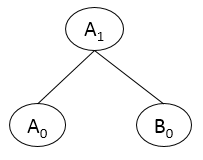
\includegraphics[width=0.2\textwidth]{commitment_tree_1.png}\\
		\caption{Possible commitment tree}
	\label{fig:figure2}
\end{figure}

\section{Aggregator can not cheat}

In this scenrio due to collision free hash fucntions, aggregator can not cheat. It means if an aggregator tries to chage the reported values by its children, their childrent will detect those values during the verification phase. 

\begin{figure}[t]
	\centering
		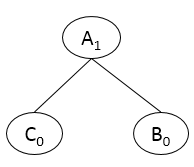
\includegraphics[width=0.2\textwidth]{commitment_tree_2.png}
		\caption{Possible commitment tree}
	\label{fig:figure2}
\end{figure}
